
% Figure 3: D3 Cross-Domain Performance (LaTeX TikZ)
\begin{figure}[ht]
\centering
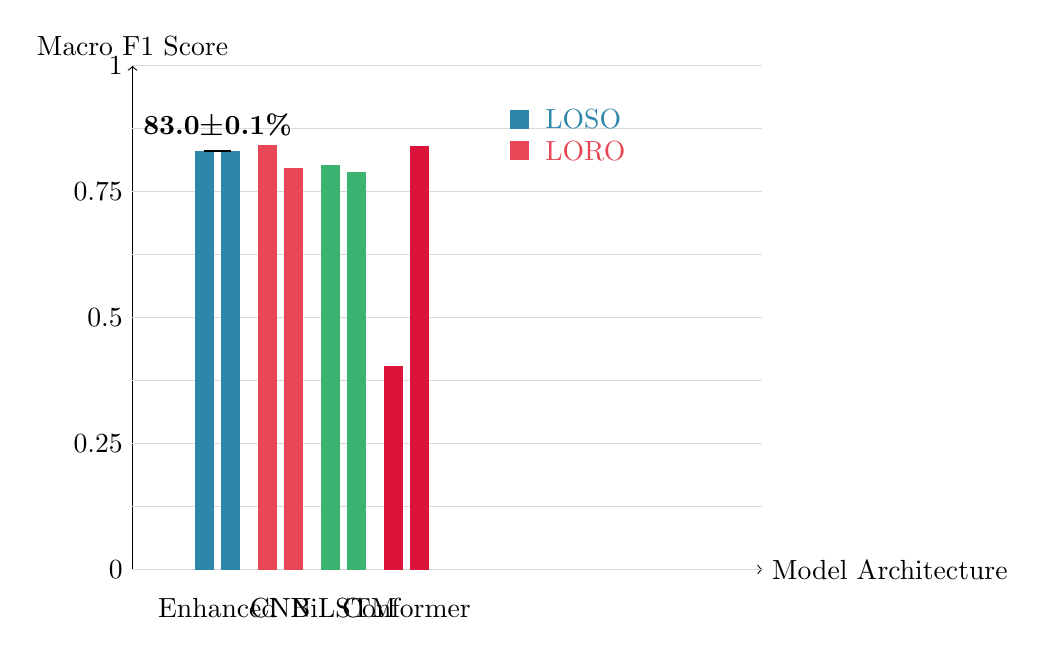
\begin{tikzpicture}[scale=0.8]
    % Define colors
    \definecolor{enhanced}{RGB}{46,134,171}
    \definecolor{cnn}{RGB}{232,72,85}
    \definecolor{bilstm}{RGB}{60,179,113}
    \definecolor{conformer}{RGB}{220,20,60}
    
    % Axes
    \draw[->] (0,0) -- (10,0) node[right] {Model Architecture};
    \draw[->] (0,0) -- (0,8) node[above] {Macro F1 Score};
    
    % Y-axis labels
    \foreach \y in {0,1,2,3,4,5,6,7,8}
        \draw[gray!30] (0,\y) -- (10,\y);
    \foreach \y in {0,2,4,6,8}
        \node[left] at (0,\y) {\pgfmathparse{\y/8}\pgfmathprintnumber{\pgfmathresult}};
    
    % LOSO bars (left group)
    \fill[enhanced] (1,0) rectangle (1.3,6.64);    % 0.830
    \fill[cnn] (2,0) rectangle (2.3,6.736);        % 0.842  
    \fill[bilstm] (3,0) rectangle (3.3,6.424);     % 0.803
    \fill[conformer] (4,0) rectangle (4.3,3.224);  % 0.403
    
    % LORO bars (right group)
    \fill[enhanced] (1.4,0) rectangle (1.7,6.64);  % 0.830
    \fill[cnn] (2.4,0) rectangle (2.7,6.368);      % 0.796
    \fill[bilstm] (3.4,0) rectangle (3.7,6.312);   % 0.789
    \fill[conformer] (4.4,0) rectangle (4.7,6.728); % 0.841
    
    % Error bars and labels
    % Enhanced (key highlight)
    \draw[thick] (1.15,6.64) -- (1.15,6.648) -- (1.55,6.648) -- (1.55,6.64);
    \node[above] at (1.35,6.7) {\textbf{83.0±0.1\%}};
    
    % Model labels
    \node[below] at (1.35,-0.3) {Enhanced};
    \node[below] at (2.35,-0.3) {CNN};
    \node[below] at (3.35,-0.3) {BiLSTM};
    \node[below] at (4.35,-0.3) {Conformer};
    
    % Legend
    \fill[enhanced] (6,7) rectangle (6.3,7.3) node[right] at (6.4,7.15) {LOSO};
    \fill[cnn] (6,6.5) rectangle (6.3,6.8) node[right] at (6.4,6.65) {LORO};
    
\end{tikzpicture}
\caption{Cross-domain generalization performance across LOSO and LORO protocols.}
\label{fig:cross_domain}
\end{figure}
